% begin module orthogonal-trajectory-def
\begin{frame}
\frametitle{Orthogonal Trajectories}
\begin{definition}[Orthogonal Trajectory]
An orthogonal trajectory to a family of curves is a curve that intersects each curve of the family orthogonally (that is, at right angles).
\end{definition}

\begin{columns}[c]
\column{.5\textwidth}
\ \uncover<2->{%
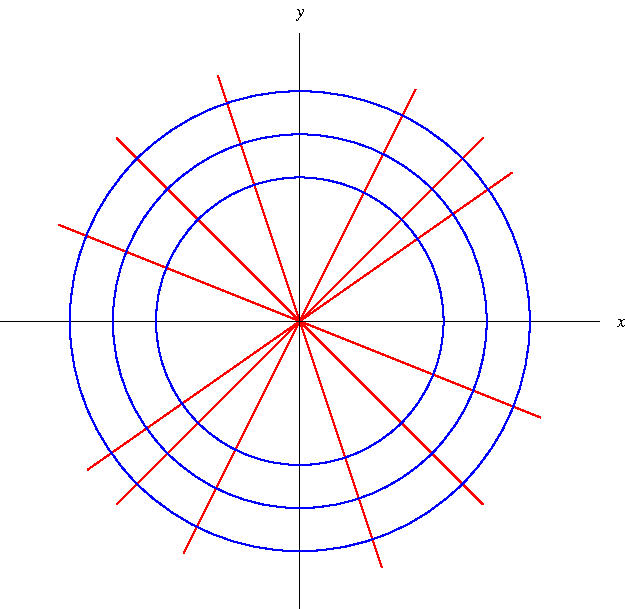
\includegraphics[height=5.5cm]{diff-eq-separable/pictures/10-03-orthcirc.pdf}%
}%
\column{.5\textwidth}
\uncover<2->{%
Each member of the family $y = mx$ of straight lines passing through the origin is an orthogonal trajectory to the family $x^2 + y^2 = r^2$ of circles centered at the origin.
}%
\end{columns}
\end{frame}
% end module orthogonal-trajectory-def
